% !TEX root = main.tex
\chapter{序論}
\section{研究背景}
\subsection{半導体レーザーからの超短光パルス発生}
\subsubsection{様々な短パルス発生法}
半導体レーザーは産業的に広く普及している発光素子である。小型化可能、大量生産可能、熱や振動(安定性)に強いことなどが主な理由である。さらに半導体から直接ピコ秒程度の超短光パルスを発生させる技術も研究が盛んに行われており、産業への応用が期待されている。
%[利得スイッチングsds生物発光yokoyamaさん,ここではGSにこだわらなくてもいいか][psパルスを使った産業]

 半導体から短パルスを発生させる方法として従来行われてきた方法が主に3つある。モード同期法、Qスイッチ法、利得スイッチ法である。モード同期法は個体レーザーでも用いられておりフーリエ限界に近いパルス幅を生成できる反面パルスの繰り返し周期が固定されてしまうという特徴を持つ。一方Qスイッチング法は過飽和吸収帯を用いるなどしてQ値を瞬間的に増大させることで高エネルギーの光パルスを得ることができる。利得スイッチングは複雑な構造を必要とせず、全ての半導体レーザーで実現が可能な技術であり実用性に秀でている。レーザー加工などの技術的応用においては繰り返し可変であることや様々な種類の光源を試すことができるという利点があるため、??本研究では利得スイッチング法に着目した。
\subsubsection{利得スイッチング法}
利得スイッチングはこの右下の図は過去40年間に行われてきた利得スイッチングのパルス幅をプロットしたものです。赤が光励起、青が電流注入を表しています。今回意図しているのは電流注入であるため、青を見てみると最短でも5psであることがわかります。この限界に挑戦したいというのがモチベーションです。[伊藤さん論文]
\subsubsection{利得スイッチング光パルスの短パルス化}
まずは利得スイッチングのメカニズムについて説明いたします。
利得スイッチングとは半導体にns以下の時間内に強く励起することで半導体内にできたキャリアが一気に放出される現象です。右の図は上から順に励起パルス、発光パルスおよび利得の時間発展の計算結果を表したものです。
電流注入に関する青いプロットを見ていただくと長い励起パルスを引火すると、利得が上がっていき、発振閾値を超えたところでキャリアを使って20ps程度の短いパルスが出てきます。

ではどのような半導体ならば短いパルスが出てくるのかという疑問に達しますがこのような先行研究がなされています。この2つの連立方程式はそれぞれキャリアとフォトンの時間変位を記述するレート方程式です。先ほどのシミュレーションも同等の式に従って計算されたものです。この研究の中ではキャリアのフォトンへの変換効率に寄与するgというファクターが高いほど発生パルスが短くなるということが示唆され、実験的に示されました。


\subsection{InGaAs高利得材料}
\

\begin{figure}[t]
	\centering
	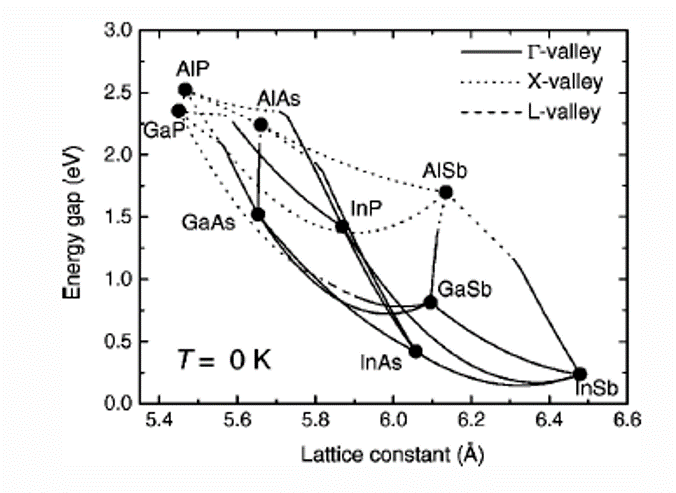
\includegraphics[width=15cm]{figure/fig_1_1_lattice_constance.png}
	\caption{格子定数}
	\label{fig:fig_latice_constancce}
\end{figure}


@歪み補償
InGaAsを用いる理由
InGaAs

\section{本研究の目的}
電流注入により短いパルスを達成すること?
新しい構造を作ったからそれを図ること?
